\documentclass[10pt,a4paper]{article}
\usepackage[margin=1.8cm]{geometry}
\usepackage{amsmath,amssymb}
\usepackage{graphicx}
\usepackage{booktabs}
\usepackage{caption}
\makeatletter
\captionsetup{font=small,labelfont=bf}
\let\olditemize\itemize \renewcommand\itemize{\olditemize\setlength\itemsep{1pt}\setlength\parskip{0pt}}
\let\oldenumerate\enumerate \renewcommand\enumerate{\oldenumerate\setlength\itemsep{1pt}\setlength\parskip{0pt}}
\setlength{\parskip}{3pt}
\setlength{\parindent}{0pt}
\renewcommand\section{\@startsection{section}{1}{0pt}{8pt plus 2pt}{3pt}{\large\bfseries}}

\makeatother
\title{\vspace{-1.6cm}\Large\bfseries Task 1 -- Development of the Blade Structural Optimisation Code}
\author{}
\date{\vspace{-1.2cm}}

\begin{document}
\maketitle

\section*{1\quad Starting point: a solver wrapper}
The brief supplies \texttt{beamBending}, an Euler--Bernoulli cantilever solver that
takes the second moment of area $I$ at $N=100$ spanwise nodes and returns the
deflection $\delta(r)$ and bending moment $M(r)$ under the worst-case load
$L_z(r)=50r\,(1-e^{50(r-R)})$. Everything else (the cross-section, the volume and the
stress check) had to be built around it. The first script, \texttt{RunBeamBending.m},
therefore has one job: turn a structural concept into the vector $I(r)$ and the area
$A(r)$, call the solver once, and report the volume $V=\int_0^R A\,\mathrm{d}r$, the tip
deflection and the peak bending stress $\sigma=|M|\,y_{\max}/I$. Following the
``start simple'' advice, the first concept was a single solid spar whose width tapers
linearly from root to tip.

\section*{2\quad Choosing the structural concept: spar vs.\ skin}
Two section models were coded behind a single switch, so that both concepts go through
the same solver, stress check and plots:
\begin{itemize}
  \item \textbf{Approach 1 -- solid spar.} The spar, centred at $x/c=0.3$ (maximum
  thickness), is split into 50 vertical strips of height $2y_t(x)$ from the NACA\,0012
  equation, giving $I=\sum b_i d_i^3/12$ and $A=\sum b_i d_i$.
  \item \textbf{Approach 2 -- thin structural skin} ($t\ll c$). Each surface is split into
  200 straight panels with cosine spacing, which concentrates panels round the
  strongly curved leading edge. Each panel contributes
  $L^3t\sin^2\theta/12 + (Lt)\,d^2$ (parallel axis theorem); the lower surface mirrors
  the upper.
\end{itemize}
A key observation from coding Approach 2 is that the skin's section properties are
\emph{linear in thickness}: $I=I_u\,t$ and $A=P\,t$, where $I_u$ and the perimeter $P$
are fixed by the aerofoil shape. They are computed once and then scaled.

With hand-picked linear tapers sized to sit just under yield, the skin carried the load
with 367\,cm$^3$ of material against 535\,cm$^3$ for the spar (31\,\% less), at
the same peak stress of 29.6\,MPa. This is what the definition $I=\int y^2\,\mathrm{d}A$
predicts: the skin places all of its material at the outer fibre, whereas the solid
spar puts much of its material near the neutral axis, where it adds area but little
stiffness. The skin was therefore taken forward to optimisation.

\section*{3\quad Making each evaluation almost free}
The brief asks for a tool that can be rerun for thousands of regions, so evaluation
cost mattered more than anything else. Two properties of the problem remove the solver
from the optimisation loop entirely:
\begin{enumerate}
  \item \textbf{The blade is statically determinate.} $M(r)$ follows from equilibrium
  alone and does not depend on $I$. One call to \texttt{beamBending} (with any $I$)
  gives $M(r)$ for \emph{every} design.
  \item \textbf{Unit-load (virtual work) method.} With $M$ known, the tip deflection is
  a single integral,
  \begin{equation}
    \delta_{\mathrm{tip}}=\int_0^R \frac{|M(r)|\,(R-r)}{E\,I(r)}\,\mathrm{d}r ,
  \end{equation}
  where $(R-r)$ is the moment due to a unit tip load. It agrees with the full solver
  to within 0.02\,\% (e.g.\ 0.6282\,m vs.\ 0.6281\,m); this check is rerun
  automatically at three points on every front.
\end{enumerate}
Together these turn each design evaluation into a handful of vector operations. The
complete Pareto front of 15 optimisations takes 1.3\,s and needs exactly one
solver call.

\section*{4\quad Formulating the optimisation}
The skin thickness was parameterised by its root and tip values,
$t(r)=t_{\mathrm{root}}+(t_{\mathrm{tip}}-t_{\mathrm{root}})\,r/R$: two variables,
consistent with the bending moment falling from root to tip. The brief asks for minimum
material, while a turbine blade also has to stay stiff. Rather than combine the two
with arbitrary weights, the trade-off was mapped as a Pareto front using the
$\varepsilon$-constraint method, which gives evenly spaced points and, unlike a weighted
sum, would also capture a non-convex front:
\begin{equation}
  \min_{t_{\mathrm{root}},\,t_{\mathrm{tip}}} V
  \quad\text{s.t.}\quad
  \frac{\sigma_{\max}}{\sigma_{\mathrm{allow}}}-1\le 0,\qquad
  \frac{\delta_{\mathrm{tip}}}{\varepsilon}-1\le 0,\qquad
  0.8\,\mathrm{mm}\le t\le 2.0\,\mathrm{mm}.
\end{equation}
Each decision has a stated reason:
\begin{itemize}
  \item $\sigma_{\mathrm{allow}}=30$\,MPa$/1.5=20$\,MPa. The safety factor covers
  print-quality scatter and the unmodelled shear stresses.
  \item The upper bound keeps $t\lesssim 20\,\%$ of the 9\,mm half-depth, so the
  thin-wall model stays valid.
  \item The lower bound is two 0.4\,mm printed perimeters, the minimum for a
  structural wall.
  \item Constraints are normalised, so that \texttt{fmincon} sees terms of order one.
\end{itemize}

\begin{center}
\fbox{\begin{minipage}{0.94\textwidth}\small
\textbf{Algorithm 1} Pareto front generation (\texttt{ParetoSkin.m})\\[-6pt]
\rule{\linewidth}{0.4pt}
\begin{tabbing}
\hspace{1.4em}\=\hspace{1.4em}\=\kill
1\> $M(r)\gets$ \texttt{beamBending}$(N,\,I_{\text{dummy}})$ \hfill \textit{only solver call}\\
2\> $\mathbf{x}_{\text{light}}\gets\arg\min V$ s.t.\ stress only;\quad $\delta_{\text{light}}\gets\delta(\mathbf{x}_{\text{light}})$ \hfill \textit{anchor 1}\\
3\> $\delta_{\text{stiff}}\gets\delta(t_{\max},t_{\max})$;\quad $\mathbf{x}_0\gets(t_{\max},t_{\max})$ \hfill \textit{anchor 2}\\
4\> \textbf{for} $\varepsilon$ in \texttt{linspace}$(\delta_{\text{stiff}},\delta_{\text{light}},15)$ \textbf{do}\\
5\>\> $\mathbf{x}^*\gets$ \texttt{fmincon}($V$, $\mathbf{x}_0$, stress \& $\delta\le\varepsilon$);\quad $\mathbf{x}_0\gets\mathbf{x}^*$ \hfill \textit{warm start}\\
6\>\> $\mathbf{x}_{\text{print}}\gets$ round $t(r)$ \emph{up} to multiples of 0.4\,mm\\
7\> \textbf{end for}\\
8\> Validate: compare $\delta$ with \texttt{beamBending}; plot the front over a $30\times30$ brute-force grid
\end{tabbing}\vspace{-8pt}
\end{minipage}}
\end{center}

\section*{5\quad Designing for the printer}
A continuous optimum such as $t=1.78$\,mm cannot be printed: an FDM wall is a whole
number of 0.4\,mm extrusion lines. Each optimum is therefore rounded \emph{up} to the
next perimeter. Rounding up only ever adds material, so the stress constraint stays
satisfied and the deflection can only fall, and no re-optimisation is needed. Two
printable designs are compared with the bounds in Table~\ref{tab:results}. The
continuous front is the real physical trade-off; the printable front (blue in
Fig.~\ref{fig:front}) is what the company can actually make.

\begin{figure}[h]
  \centering
  \begin{minipage}{0.56\textwidth}
    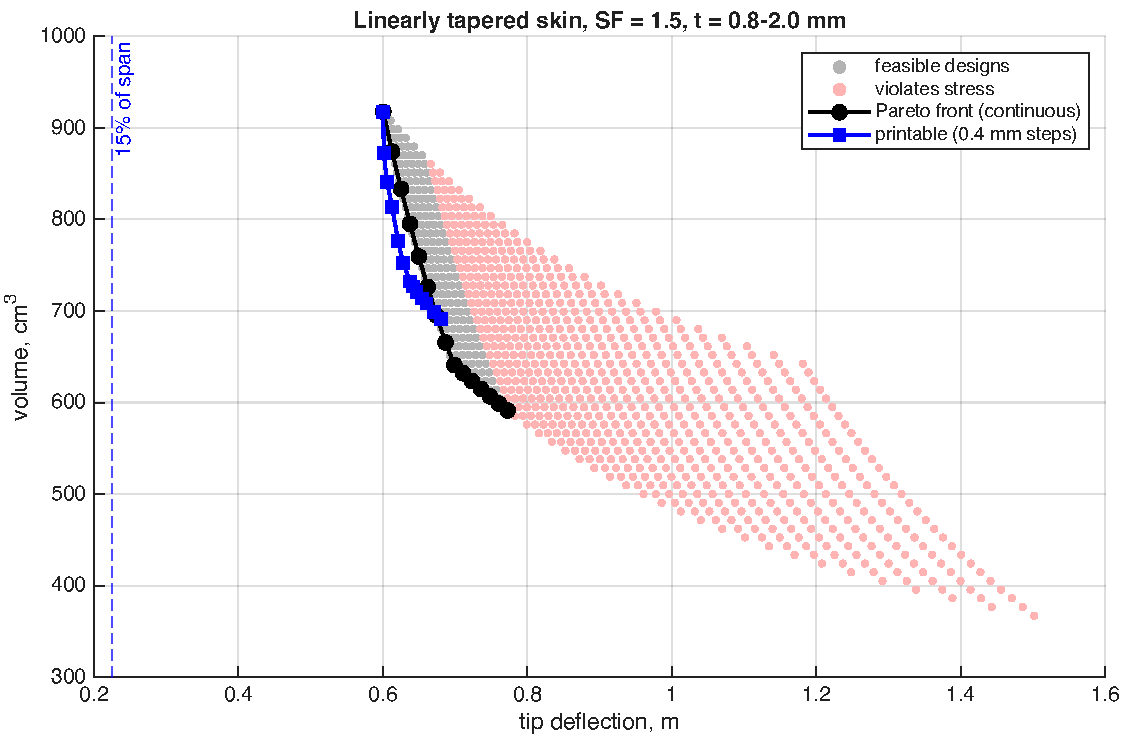
\includegraphics[width=\linewidth]{pareto_front.pdf}
  \end{minipage}\hfill
  \begin{minipage}{0.41\textwidth}
    \captionof{figure}{Volume vs.\ tip deflection for the linearly tapered skin. Grey
    and red dots: brute-force grid (stress-feasible and infeasible). Black: continuous
    $\varepsilon$-constraint front, which lies on the edge of the feasible grid and so
    confirms that \texttt{fmincon} converged to the true optima. Blue: printable
    designs after rounding up to whole perimeters.}
    \label{fig:front}
    \vspace{6pt}
    \small
    \captionof{table}{Bounds of the continuous front (top) and two printable designs (bottom).}
    \label{tab:results}
    \begin{tabular}{@{}lccc@{}}
      \toprule
      Design & $V$ (cm$^3$) & $\delta_{\text{tip}}$ (m) & $t_{\text{root}}/t_{\text{tip}}$ (mm)\\
      \midrule
      Lightest   & 591 & 0.77 & 1.78 / 0.80 \\
      Stiffest   & 918 & 0.60 & 2.00 / 2.00 \\
      \midrule
      Lightest   & 692 & 0.68 & 2.0 / 0.8 \\
      Point 8    & 753 & 0.63 & 2.0 / 1.2 \\
      \bottomrule
    \end{tabular}
  \end{minipage}
\end{figure}

\section*{6\quad What the results show so far}
\begin{itemize}
  \item \textbf{The optima behave as expected.} Along the front, material is first
  removed from the tip, where the moment is small. Once $t_{\mathrm{tip}}$ reaches the
  0.8\,mm print limit ($V\approx641$\,cm$^3$), only the root can thin further,
  which creates the kink in the front. At the lightest point the stress constraint is
  exactly active at the root.
  \item \textbf{Printing costs material.} Rounding to whole perimeters adds 17\,\% to the
  lightest design (591 $\to$ 692\,cm$^3$). It also collapses the three stiffest
  points onto one design, because 1.6--2.0\,mm all round to the same perimeter count.
  This rounding loss is now one of the largest sources of inefficiency.
  \item \textbf{Stiffness is the limiting physics.} Every design deflects 0.60--0.77\,m,
  40--50\,\% of the span. This is far from the 15\,\% guideline and outside the
  small-deflection validity of Euler--Bernoulli theory. A thin ABS skin limited to
  2\,mm is strength-adequate but not stiff enough.
\end{itemize}

\section*{7\quad Next steps}
\begin{itemize}
  \item \textbf{Non-linear thickness distributions.} Try a power law and pchip control
  points. Because $I\propto t$, the problem is convex, and the optimality conditions give
  $t^*(r)\propto\sqrt{|M|(R-r)}$, clipped by the stress and print limits. This is an
  analytic benchmark that any parameterisation can be measured against.
  \item \textbf{Optimise the number of perimeters per zone directly.} Treating perimeter
  counts as integers (\texttt{ga} with \texttt{IntCon}) would remove the rounding loss.
  \item \textbf{Address the stiffness deficit.} Relax $t_{\max}$ with a thick-wall
  section, or combine the skin with a spar (Approach 1\,+\,2).
\end{itemize}

\end{document}
